\documentclass[12pt, letterpaper]{article}
\usepackage{amsmath,amssymb} % math mode
\usepackage{bm} % bold vector notation
\usepackage{graphicx} % figures
\usepackage{mathrsfs} % script letters

\DeclareMathOperator{\cov}{\text{cov}}
\DeclareMathOperator{\cor}{\text{cor}}
\DeclareMathOperator{\var}{\text{var}}
\DeclareMathOperator{\diag}{\text{diag}}
\DeclareMathOperator{\tr}{\text{tr}}
\DeclareMathOperator{\clr}{\text{clr}}

\setlength{\parindent}{0em}
\setlength{\parskip}{1em}

\begin{document}

\section{Background}

Basis abundances:
\begin{equation}
\bm{w} = (w_1, \dots, w_D) \in \mathscr{R}_+^D
\end{equation}

Composition:
\begin{equation}
\bm{x} = (x_1, \dots, x_D) = \mathscr{C}(\bm{w}) = \bm{w} / (w_1 + \dots + w_D) \in \mathscr{S}^d
\end{equation}

Centered log-ratios:
\begin{align}
\bm{z} = \clr(\bm{x}) &= \log(\bm{x} / g(\bm{x})) = \log(\bm{w} / g(\bm{w})),\ g(\bm{x}) = \left(\prod_i x_i\right)^{1/D} \\
&= \left( \log x_1 - \frac{1}{D} \sum_i \log x_i, \dots, \log x_D - \frac{1}{D} \sum_i \log x_i \right) \\
&= \left( \log w_1 - \frac{1}{D} \sum_i \log w_i, \dots, \log w_D - \frac{1}{D} \sum_i \log w_i \right)
\end{align}

Log-ratio variances:
\begin{equation}
\tau_{ij} = \var \log(x_i / x_j)
\end{equation}

Basis covariances:
\begin{equation}
\var(\log \bm{w}) = \bm{\Omega}
\end{equation}

Centered log-ratio covariances:
\begin{equation}
\var(\clr \bm{x}) = \var(\clr \bm{w}) = \bm{\Gamma}
\end{equation}

Variation matrix:
\begin{equation}
\left[ \tau_{ij} \right] = \left[ \var(\log(x_i / x_j)) \right] = \bm{T}
\end{equation}

$\bm{\Omega} \rightarrow \bm{\Gamma}$:
\begin{align}
\gamma_{ij} &= \omega_{ij} - \omega_{i\cdot} - \omega_{j\cdot} + \omega_{\cdot\cdot} \\
\bm{\Gamma} &= \bm{G} \bm{\Omega} \bm{G},\ \bm{G} = \bm{I} - D^{-1}\bm{J},\ \bm{J} = \left[ 1 \right]_{D \times D}
\end{align}

$\bm{\Omega} \rightarrow \bm{T}$:
\begin{align}
\tau_{ij} &= \omega_{ii} + \omega_{jj} - 2\omega_{ij} \\
\bm{T} &= \bm{J}\diag(\bm{\Omega}) + \diag(\bm{\Omega})\bm{J} - 2\bm{\Omega}
\end{align}

$\bm{\Gamma} \leftrightarrow \bm{T}$:
\begin{align}
\tau_{ij} &= \gamma_{ii} + \gamma_{jj} - 2\gamma_{ij} \\
\bm{T} &= \bm{J}\diag(\bm{\Gamma}) + \diag(\bm{\Gamma})\bm{J} - 2\bm{\Gamma} \\
\gamma_{ij} &= \frac{1}{2}(\tau_{i\cdot} + \tau_{j\cdot} - \tau_{ij} - \tau_{\cdot\cdot}) \\
\bm{\Gamma} &= -\frac{1}{2}\bm{G}\bm{T}\bm{G}
\end{align}

\section{Findings}

$\bm{\Gamma} \rightarrow \bm{\Omega}$ parameterized by $\omega_{11}, \dots, \omega_{DD}$:
\begin{align}
\omega_{ij} &= \frac{1}{2} \left( \omega_{ii} + \omega_{jj} - \tau_{ij} \right) \\
&= \frac{1}{2} \left( \omega_{ii} + \omega_{jj} - \gamma_{ii} - \gamma_{jj} + 2\gamma_{ij} \right) \\
&= \gamma_{ij} + \frac{1}{2} \left( \omega_{ii} - \gamma_{ii} + \omega_{jj} - \gamma_{jj} \right) \\
\bm{\Omega} &= \frac{1}{2} \left( \bm{J}\diag(\bm{\Omega}) + \diag(\bm{\Omega})\bm{J} - \bm{T} \right) \\
&= \frac{1}{2} \left( \bm{J}\diag(\bm{\Omega}) + \diag(\bm{\Omega})\bm{J} - \bm{J}\diag(\bm{\Gamma}) - \diag(\bm{\Gamma})\bm{J} + 2\bm{\Gamma} \right) \\
&= \bm{\Gamma} + \frac{1}{2} \left[ \bm{J} \left( \diag(\bm{\Omega}) - \diag(\bm{\Gamma}) \right) + \left(\diag(\bm{\Omega}) - \diag(\bm{\Gamma}) \right)\bm{J} \right]
\end{align}

Notation for set of potential basis covariances associated with a given clr covariance matrix:
\begin{equation}
\mathscr{B}(\bm{\Gamma}) = \{ \bm{\Omega}: \bm{\Omega} \text{ is symmetric positive semi-definite and } \bm{G}\bm{\Omega}\bm{G} = \bm{\Gamma} \}
\end{equation}

$\bm{\Gamma}$ has minimal total variance among all $\bm{\Omega}$s which have corresponding clr covariances $\bm{\Gamma}$:
\begin{enumerate}
\item Given a clr covariance matrix $\bm{\Gamma}$, suppose there exists $\bm{\Omega} \in \mathscr{B}(\bm{\Gamma})$ such that $\tr(\bm{\Omega}) < \tr(\bm{\Gamma})$.
\item For $j = (1, \dots, 1)^\intercal$,
\begin{align}
j^\intercal \bm{\Omega} j &= \sum_i \sum_j \omega_{ij} \\
&= \sum_i \sum_j (\gamma_{ij} + \frac{1}{2}[\omega_{ii} - \gamma_{ii} + \omega_{jj} - \gamma_{jj}]) \\
&= \sum_i \left\{ 0 + \frac{1}{2} \left[ p\omega_{ii} - p\gamma_{ii} + \tr(\bm{\Omega}) - \tr(\bm{\Gamma}) \right] \right\} \\
&= \frac{1}{2} \left\{ p\tr(\bm{\Omega}) - p\tr(\bm{\Gamma}) + p\tr(\bm{\Omega}) - p\tr(\bm{\Gamma}) \right\} \\
&= \tr(\bm{\Omega}) - \tr(\bm{\Gamma}) \\
&< 0
\end{align}
\item Thus, $\tr(\bm{\Omega}) < \tr(\bm{\Gamma})$ implies that $\bm{\Omega}$ is not positive semi-definite, which contradicts the premise that $\bm{\Omega} \in \mathscr{B}(\bm{\Gamma})$.
\item Therefore, it must be that for all $\bm{\Omega} \in \mathscr{B}(\bm{\Gamma})$, $\tr(\bm{\Omega}) \geq \tr(\bm{\Gamma})$.
\end{enumerate}

For $D = 2$, it is possible to describe $\mathscr{B}(\bm{\Gamma})$ exactly. We can see which basis correlations and partial correlations are possible for a given $\bm{\Gamma}$, and visualize the structure of $\mathscr{B}(\bm{\Gamma})$.
\begin{enumerate}
\item For $D = 2$, $\bm{\Gamma}$ is completely determined by one entry because $\gamma_{11} = -\gamma_{12} = -\gamma_{21} = \gamma_{22}$. And $\gamma_{11} = \omega_{11} - \omega_{i\cdot} - \omega_{j\cdot} + \omega_{\cdot\cdot} = -\omega_{12} + \frac{1}{4}(\omega_{11} + 2\omega_{12} + \omega_{22}) = \frac{1}{4}(\omega_{11} - 2\omega_{12} + \omega_{22}) = \var[\frac{1}{2} \log(w_1/w_2)] = \frac{1}{4} \tau_{12}$.
\item Positive semi-definiteness of $\bm{\Omega}$ requires that for any $\bm{x} \in \mathscr{R}^2,\ \bm{x} \ne \bm{0}$, $\omega_{11} x_1^2 + 2\omega_{12} x_1 x_2 + \omega_{22} x_2^2 \geq 0$. First, if $x_1 = 0$ then $\omega_{22} \geq 0$, and if $x_2 = 0$ then $\omega_{11} \geq 0$. Let $x_2 \ne 0$ be fixed. Then we need the quadratic expression $\omega_{11} x_1^2 + 2\omega_{12} x_2 x_1 + \omega_{22} x_2^2 \geq 0$ for all $x_1$. That requires that the determinant $4\omega_{12}^2 x_2^2 - 4\omega_{11}\omega_{22} x_2^2 = 4x_2^2 (\omega_{12}^2 - \omega_{11}\omega_{22}) \leq 0$ which requires that $\omega_{12}^2 - \omega_{11}\omega_{22} \leq 0$.
\item $\omega_{12} = \gamma_{12} + \frac{1}{2}(\omega_{11} - \gamma_{11} + \omega_{22} - \gamma_{22}) = -\gamma_{11} + \frac{1}{2}\omega_{11} - \frac{1}{2}\gamma_{11} + \frac{1}{2}\omega_{22} -  \frac{1}{2}\gamma_{11} = \frac{1}{2}(\omega_{11} + \omega_{22}) - 2\gamma_{11}$.
\item $\omega_{12}^2 - \omega_{11}\omega_{22} = \frac{1}{4}\omega_{22}^2 - (\frac{1}{2}\omega_{11} + 2\gamma_{11})\omega_{22} + (\frac{1}{4}\omega_{11}^2 - 2\gamma_{11}\omega_{11} + 4\gamma_{11}^2) = 0$ when $\omega_{22} = \left[ \frac{1}{2}\omega_{11} + 2\gamma_{11} \pm 2\sqrt{\gamma_{11}\omega_{11}} \right] / \frac{1}{2} = (\sqrt{\omega_{11}} \pm 2\sqrt{\gamma_{11}})^2$.
\item $\omega_{12}^2 - \omega_{11}\omega_{22} \leq 0$ when $(\sqrt{\omega_{11}} - 2\sqrt{\gamma_{11}})^2 \leq \omega_{22} \leq (\sqrt{\omega_{11}} + 2\sqrt{\gamma_{11}})^2$. In combination with $\omega_{12} = \frac{1}{2}(\omega_{11} + \omega_{22}) - 2\gamma_{11}$, this defines $\mathscr{B}(\bm{\Gamma})$ for $D = 2$.
\item Within the set $\mathscr{B}(\bm{\Gamma})$, what basis correlations are possible? $\omega_{12} = 0$ when $\omega_{22} = 4\gamma_{11} - \omega_{11}$, $\omega_{12} < 0$ when $\omega_{22} < 4\gamma_{11} - \omega_{11}$, and $\omega_{12} > 0$ when $\omega_{22} > 4\gamma_{11} - \omega_{11}$. In particular, $\omega_{12}^2 = \omega_{11}\omega_{22}$ (i.e. $\rho_{12} = \pm 1$) along the line bounding the set. Here the partial correlations are the same as the marginal correlations.
\item $\bm{\Gamma}$ is at the ``vertex" of the set $\mathscr{B}(\bm{\Gamma})$.
\end{enumerate}

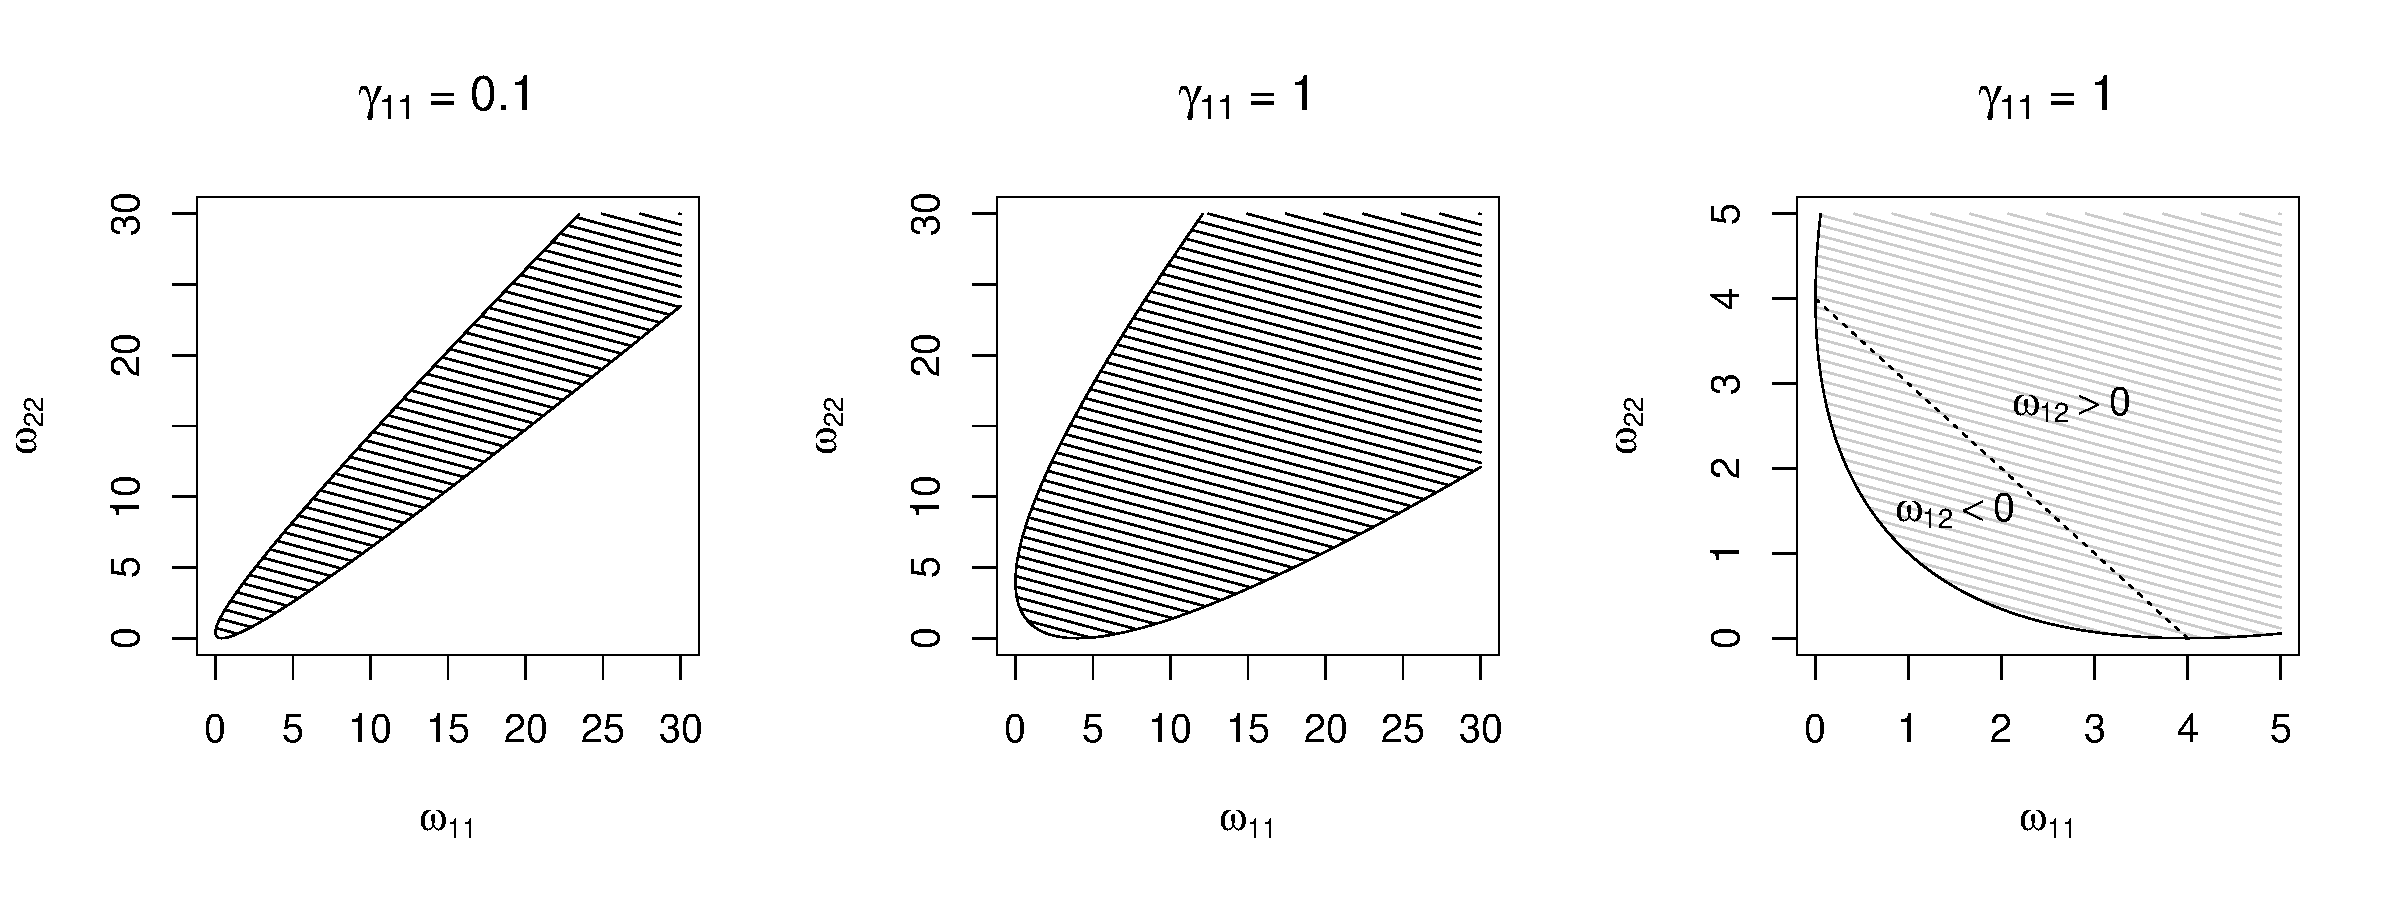
\includegraphics[width=5.5in]{figures/D2regions.pdf}

For any $D \geq 2$, given $\bm{\Gamma}$, there exists $\bm{\Omega} \in \mathscr{B}(\bm{\Gamma})$ in which $\omega_{ij} > 0$ and there exists $\bm{\Omega} \in \mathscr{B}(\bm{\Gamma})$ in which $\omega_{ij} < 0$, provided $\tau_{ij} > 0$. (A particular basis correlation always could be either negative or positive if there are no restrictions on $\bm{\Omega}$ and $\var[\log(x_i / x_j)] > 0$.)
\begin{enumerate}
\item First, $\omega_{ij}$ can be $> 0$: For clr data $\bm{z} = (\clr x_1, \dots, \clr x_D)$ with covariance matrix $\bm{\Gamma}$, if $\gamma_{ij} > 0$, then $\bm{\Gamma}$ is such a $\bm{\Omega}$. If $\gamma_{ij} \leq 0$, let $\bm{y} = \bm{z} + e$ where $e$ is any random variable uncorrelated with every $z_i$ and with $\var(e) > \gamma_{ij}$. Then $\var(\bm{y}) \in \mathscr{B}(\bm{\Gamma})$ because $\clr(\bm{y}) = \bm{z}$, and $\cov(y_i, y_j) = \gamma_{ij} + \var(e) > 0$.
\item Now, $\omega_{ij}$ can be $< 0$ provided $\tau_{ij} > 0$: For clr data $\bm{z} = (\clr x_1, \dots, \clr x_D)$ with covariance matrix $\bm{\Gamma}$, if $\gamma_{ij} < 0$, then $\bm{\Gamma}$ is such a $\bm{\Omega}$. If $\gamma_{ij} \geq 0$, let $\bm{y} = \bm{z} - \frac{1}{2}(z_i + z_j)$. Then $\cov(y_i, y_j) = \cov(\frac{1}{2}\clr x_i - \frac{1}{2}\clr x_j, -\frac{1}{2}\clr x_i + \frac{1}{2}\clr x_j) = -\frac{1}{4}(\gamma_{ii} - 2\gamma_{ij} + \gamma_{jj}) = \frac{1}{4}\tau_{ij} < 0$ and in fact $\var(y_i) = \var(y_j) = \frac{1}{4}\tau_{ij}$, so $\cor(y_i, y_j) = -1$.
\end{enumerate}

For $D > 2$, based on empirical investigation, any value is possible for a given partial correlation if there are no restrictions on $\bm{\Omega}$.

For a given $\bm{\Gamma}$, potential $\bm{\Omega}$s can be randomly generated within the set constrained by $\tr(\bm{\Omega}) \leq V_{max}$.
\begin{enumerate}
\item Generate a random unit-length vector $\bm{a}$ using a re-scaled $D$-dimensional normal(0, 1) vector.
\item Let $\bm{z} = (z_1, \dots, z_D)^\intercal$ be the clr vector. Calculate maximum $r$ such that $\sum_{i=1}^D \var(z_i + r \bm{a}^\intercal \bm{z}) \leq V_{max}$. Call that $r_{max}$.
\item Generate a random $r$ from the uniform(0, $r_{max}$) distribution.
\item Calculate $v_{max} = V_{max} - \sum_{i=1}^D \var(z_i + r \bm{a}^\intercal \bm{z})$.
\item Generate a random $v$ from the uniform(0, $v_{max}$) distribution.
\item Let the log abundances be $y_i = z_i + r \bm{a}^\intercal \bm{z} + e$ where $e$ is an independent random variable with $\var(e) = v$.
\item Then $\bm{\Omega} = \bm{\Gamma} + r \bm{\Gamma} \bm{A} + r \bm{A}^\intercal \bm{\Gamma} + r^2\bm{A}^\intercal \bm{\Gamma} \bm{A} + v\bm{J}$.
\end{enumerate}

\end{document}